\chapter{Theoretical predictions and event simulation}
\label{ch:simulation}

Quantifying the agreement of experimental observations with the SM
or with possible BSM theories is a core goal of collider physics.
While the SM is a nearly complete and profoundly successful theory,
connecting theories that concern the interactions and excitations of quantum fields
to the electrical signals induced in the CMS detector by
\pp collisions is highly non-trivial.
In an ideal case, one would use
the theory of particles and fields outlined in Chapters~\ref{ch:introduction} 
and 2 %\ref{ch:phenomenology} 
as input to derive the expected distribution
of measurable signals resulting from \pp collisions.
In this paradigm, BSM modifications to the SM are realized as modifications 
to the structure of the underlying QFT. They lead to new interactions, which
modify the rate or type of particle production, or kinematics variables 
of the produced particles, leading to deviations from the SM expectation
in measured quantities. 
In practice, a factorized approach---leveraging approximations and tuning 
to experimental data---allows the simulation of primary particle production in
\pp collisions, the formation of bound states and particle decay,
and the interactions of particles in the CMS detector 
to be simulated in a way that largely achieves this goal.
The CMS Collaboration benefits from the work of collaborations of theoretical 
physicists and many previous studies to produced the detailed simulations
used to model signal and background processes for this analysis.

Nonetheless, it is important to highlight that the experimental physicists
is not purely at the mercy of the simulations from which our predictions derive.
Many predictions are phenomenological in nature, i.e., they have been tuned to the 
observations measured in LHC collisions and previous accelerators.
Furthermore, in situ measurements allow the data observation 
to modify aspects of the predictions. Lastly, broad knowledge of the nature
of particle production in collisions can sometimes be leveraged to completely 
remove dependence on simulation. For example, with no resonant source of 
diphoton production, the $m_{\gamma\gamma}$ distribution would be a falling spectrum.
The first measurements of the scalar Higgs boson with $m_{\PH} = 125\GeV$ made 
in the diphoton channel where achieved with the SM $\pp\to\gamma\gamma$ 
expectation parameterized as a falling exponential distribution,
not with an ab initio simulation of the distribution~\cite{Aad:2014eha,Khachatryan:2014ira}.

The results in this thesis exploit the data constrain important backgrounds.
However, the \EWWZ and \QCDWZ processes are only distinguishable by their kinematic
distributions, which cannot be independently observed. 
Determining the production mechanism
of {\WZjj} production and identifying the component that is sensitive to the
\WWZZ coupling relies heavily on achieving well-understood simulations of the
signal and background processes contributing to the events analyzed.
This chapter discusses the techniques used to simulate \pp collisions at the
LHC. The techniques used to obtain results for \WZjj production in the SM and beyond,
and the predictions used in this analysis, are presented and discussed.

\section{Anatomy of an LHC collision}

As discussed in Chapter~\ref{ch:phenomenology}, perturbation theory is the 
most effective technique for calculations of particle scattering in
the SM QFT. While the underlying principles are well-established, calculations
of QCD interactions, in particular, are computationally challenging. The QCD 
theory is asymptotically free, meaning $\alpha_s(\mu)$ grows with low values of 
the energy scale $\mu$, so low-energy phenomena are non-perturbative.
Because asymptotic freedom also leads to bound states at the low 
energy scales of most physical phenomena, the energy regime of stable particles---and
therefore the incoming state directed to collision and the outgoing particles
that interact with the detector---have non-perturbative properties.

The uncomfortable dichotomy between the regime of most physical phenomena and calculability
is averted by the concept of factorization, which allows a separation of short-distance
interactions from long-distance interactions, or equivalently, interactions governed
by energy scales large or small with respect to $\lqcd\approx 200\MeV$.
Factorization states that the interaction
of hadrons can be reduced to structure functions describing the distribution of quarks
and gluons in hadrons, known as parton distribution functions (PDF), convoluted
with the parton-parton interaction cross section. At high momentum transfer,
the parton-parton interaction can be described perturbatively. Furthermore,
the evolution of the interaction from outgoing quarks, gluons, and leptons
can be factorized from the formation of bound states, described by 
parton-to-hadron fragmentation functions, and their decay. The concept is illustrated
for \pp collisions in Fig.~\ref{fig:factorization}.
Factorization 
is formally established under certain conditions~\cite{Collins:1989gx}, and it 
has been highly successful in describing experimental observations over generations
of hadron-hadron, lepton-lepton, and hadron-lepton colliders.

\begin{figure}[htbp]
  \centering
   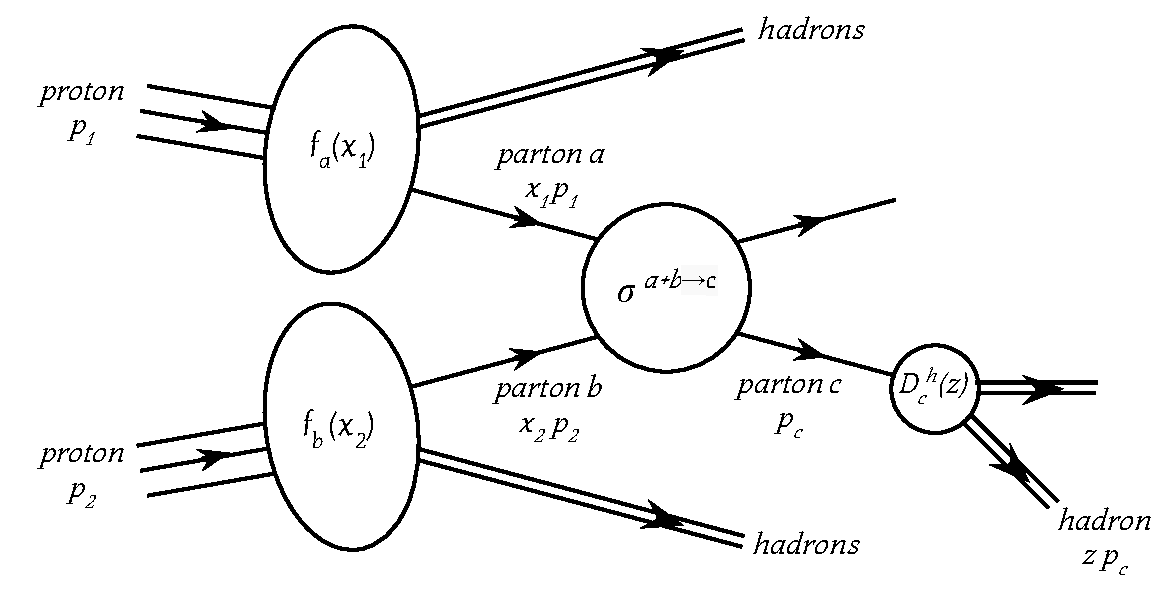
\includegraphics[width=0.6\textwidth]{figures/Simulation/factorization.pdf}
  \caption[Illustration of the principle of QCD factorization]{
    Illustration of the principle of QCD factorization. The cross section
    of the process $\pp\to X$ is reduced to the parton distribution
    functions $f_{a,b}(x)$, the partonic cross sections $\sigma^{a+b\to c}$,
    and the parton-to-hadron fragmentation functions $D_{c}^{h}(z)$.
    Reproduced from Ref.~\cite{Adare:2014hsq}.
        }
 \label{fig:factorization}
\end{figure}


Factorization allows the challenge of describing LHC collisions to be
tackled in pieces, leveraging different techniques for each piece while benefiting
from possibly independent experimental data. 
This chapter summarizes how these factorized components are modeled
for the simulations that are used to guide in this analysis.
In some cases, it is useful to consider only some contributions.
For example, the effect of the experimental
reconstruction can be parameterized by reconstruction efficiencies, or,
in cases where the effects are not dramatic and are well-established,
the hadronization
of quarks and gluons can be reduced to an effective smearing. This 
features allow calculations that neglect aspects of the full simulation
to still be used for meaningful comparisons with experimental measurements.

\section{Parton distribution functions}

A fundamental consequence of factorization is that the low-energy confinement
of quarks and gluons in the proton can be described independently from the 
parton-parton interaction in a hard collision, e.g., momentum transfer 
$Q^2 \gg \lqcd^2$. Mathematically, the 
separation of the proton structure and the high-$Q^2$ parton interaction,
shown pictorially in Fig.~\ref{fig:factorization}, can
be expressed as
\begin{equation}
  \sigma^{\pp\to X} = \sum_{a,b\in\{q,g\}}\int{\mathrm{d}x_1\mathrm{d}x_2f_{a}(x_1, \muF^{2})f_{a}(x_2,\muF^{2})}
      \hat{\sigma}^{\Pq\Pq'\to X}(x_1x_2s, \muF^{2})
\end{equation}
where $x_1$ and $x_2$ are the fractions of the proton momentum carried by 
partons $a,b \in \{q,g\}$ and the PDFs $f_{a,b}(x_i)$ give
the probability of extracting the given parton with momentum fraction $x_{i}$
from the proton.
The total momentum must be divided amongst the constituents, i.e.,
\begin{equation}
  \sum_{i}\int_{0}^{1}\mathrm{d}x xf_{i}(x, \muF^2) = 1
\end{equation}
Here $\muF$ is the factorization scale, an energy scale which represents the transition
from the non-perturbative regime of the PDF and the perturbative high $Q^2$ interaction.
Thought it is often convenient to take $\muF^2=Q^2$, $\muF$ is a free parameter that is an
artifact of the truncated serious in perturbation theory. As the order of the perturbation
expansion considered increases, the $\muF$ dependence of the result is reduced.

At least to very good approximation, the PDFs can be considered universal functions. 
Therefore, they can be derived using independent measurements, such as
deep inelastic scattering of lepton and proton beams. As shown in Fig.~\ref{fig:dis}, a lepton
incident on a proton target interacts with the quarks of the proton via a virtual
$\gamma$ or {\cPZ}. By controlling the incident energy of the proton and lepton and
measuring the outgoing particles, the abundance and momentum fraction of the proton
constituents can be established.
\begin{figure}[htbp]
  \centering
   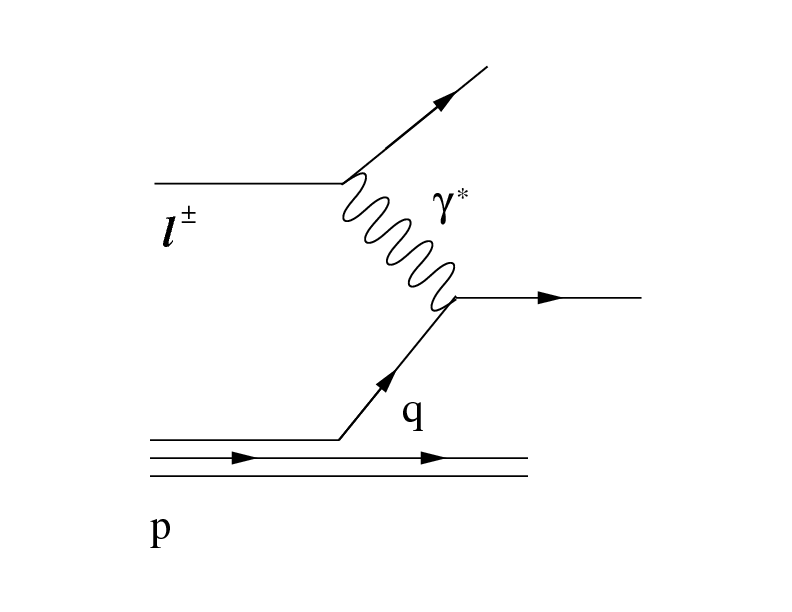
\includegraphics[width=0.5\textwidth]{figures/Simulation/DIS.png}
  \caption[Illustration of deep inelastic scattering of a lepton from a proton]{
    Illustration of deep inelastic scattering of a lepton from a proton, used
    as a probe of the internal parton structure of the proton.
    Reproduced from Ref.~\cite{Filippone:2001ux}.
        }
 \label{fig:dis}
\end{figure}

In practice, it is not feasible to parameterize all partons (and flavors) for
all $x_{i}$ through experimental measurements. Fortunately, while perturbation theory
cannot predict the formation of bound states, it does allow a means to 
parameterize the evolution of the bound partons across energy scales. The scale
dependence of the PDF is captured by the DGLAP equations, first established
by Dokshitzer~\cite{Dokshitzer:1977sg}, Gribov~\cite{Gribov:1972ri}, 
Alterelli and Parisi~\cite{Altarelli:1977zs} in the 1970s:
\begin{equation}
  \muF^2\frac{\mathrm{d}f_{a}(x, \muF^2)}{\mathrm{d}\muF^2} =
    \sum_{b\in\{q,g\}}\int_{x}^{1}\frac{\mathrm{d}z}{z}\frac{\alpha_s}{2\pi}
    \hat{P}_{ba}(z))f_b(x/z,\muF^2) \,.
\end{equation}
The functions $\hat{P}_{ba}(z)$ are the Alterelli--Parisi splitting functions,
which describe the splitting of parton $a$ into $b$, carrying a momentum
fraction $z$ of the initial momentum, that
can be derived order by order in perturbation theory. The splitting of
parton $a$ is accompanied by an additional parton, e.g., $\Pg\to\Pq\Paq$,
that is absorbed in to the parton sea of the proton. Given the DGLAP equations,
if the proton PDF can be established for any complete phase space of
parton flavors, momentum fractions, and $Q^2$, it can be evolved to all other 
scales. In practice, the contributions to the PDF are measured
at many different $Q^2$ with experiments sensitive to different quark flavors.
The experimental data is fitted, considering the DGLAP evolution, to obtain
a full parametrization of the PDF at all energy scales. 

Collaborations of theorist use independent techniques to fit data
from many collider and fixed-target experiments to produce large data sets
of predictions that can be used in simulations. The PDF is parameterized
and distributed as data grids that can be sampled with a centralized interfaced
known as LHAPDF~\cite{Buckley:2014ana}. Results in this thesis primarily
make use of the NNPDF3.0~\cite{NNPDF2015} set of PDFs, which use a neutral net to generate
pseduodata that is parameterized with global fits. 
Uncertainties in this procedure are assessed by evaluating the quality of the PDF fit to the data, 
comparing the predictions of independent collaborations
in a formulaic way~\cite{Butterworth:2015oua}, and by determining
the dependence of predictions on $\muF$.
The PDF uncertainty and its impact on the results of this thesis
are further discussed in Chapter~\ref{ch:analysis}.

\section{Perturbative calculations and matrix element generators}

With the parton content of the proton captured by the PDFs, the next challenge
in modeling an LHC collision is the perturbative calculation of the parton-parton
interaction. As discussed in Chapter~\ref{ch:phenomenology}, perturbation theory
relies on an expansion in the coupling constants of the theory,
\begin{equation}
  \sigma = \sigma_0\alpha_s^{0} + \sigma_1\alpha_s^{1} + \sigma_2\alpha_s^{2} + \cdots\,.
  \label{eq:pqcd}
\end{equation}
For a process with only by EW couplings at the lowest order, such as VV production,
$\sigma_0$ is called the leading order (LO) cross section, and $\sigma_1$ the 
next-to-leading order (NLO). 
While $\alpha_s$ is sufficiently small at the LHC collision energy to justify the
perturbative expansion ($\alpha_s(m_{\PZ}) = 0.1189 \pm 0.0010$~\cite{Tanabashi:2018oca}),
the energy and phase-space dependence of higher-order terms is non-trivial,
leading to QCD corrections much larger than the naive 
expectation in many cases~\cite{Altarelli:1979ub,Campbell:2011bn,Dittmaier:2011ti}.
The majority of production processes at the LHC require a calculation at least to NLO in QCD for percent-level accuracy.
Theoretical tools have advanced to allow automated computation of all 
SM processes at NLO~\cite{Gleisberg:2008ta,MGatNLO,Recola},
and many processes have recently been computed at NNLO in QCD~\cite{Grazzini:2017mhc}.
Calculations
at LO in the EW theory are often sufficient for percent-level accuracy. However,
some processes are susceptible to anomalously large EW corrections, including
VBS VV production~\cite{Biedermann:2016yds}, considered in this thesis.

The cross section of Equation~\ref{eq:pqcd} can be expressed in terms of the square of 
the scattering matrix element $\mathcal{M}$, which 
expresses the transition probability from the initial to the final state.
The matrix element, or scattering amplitude, is calculable in perturbation theory, of which
techniques based on Feynman diagrams are the most familiar. 
Because the total cross section is a scan over all possible outgoing energy and momenta
combinations of the outgoing particles, the cross section is an integration over a
many-dimensional phase space of configurations $\Phi_{n}$,
\begin{equation}
  \sigma_{i} = \int \mathrm{d}\Phi_{n}\left|\mathcal{M}_i\right|^2 \,.
  \label{eq:meint}
\end{equation}
The integration can be performed with numerical techniques. The high dimensionality
of the phase space, as well as the complex peak structure arising from resonances,
is well-suited for Monte Carlo (MC) integration techniques, described in the following section.

In the Feynman diagram approach to matrix-element calculations, amplitudes are represented by Feynman diagrams
where QCD (EW) coupling vertices in the diagrams are proportional to $\sqrt{\alpha_s}$ ($\sqrt{\alpha}$).
A calculation at a given perturbative order involves all diagrams connecting 
desired initial and final states for which the product of vertices is less than the order
of the perturbative expansion.
Feynman diagrams can be generated in an automated procedure with techniques from graph theory, 
before being used to derive and calculate amplitudes from Feynamn rules in the SM.
Automation of this process was established in the early 1990s at LO~\cite{Stelzer:1994ta}.
Extending this to procedure to NLO has been accomplished more recently by the 
program \MG~\cite{MGatNLO}, the successor to the previous work, which is used extensively
for MC simulations in this thesis.

Diagrams without loop contributions are called ``tree-level'' diagrams. The lowest tree-level
contribution to a given state, shown for $\pp\to\PW\PZ$ in Fig.~\ref{fig:WZNLO} (far left),
is referred to as the Born-level contribution to the process. The NLO correction to the Born
process includes contributions from tree-level diagrams of $\pp\to\PW\PZ+\jet$ for $\jet\in\{\Pg,\Pq\}$, 
known as real emission diagrams, and loop contributions, shown in Fig.~\ref{fig:WZNLO} (center)
and (left) respectively. 
Divergences from each of these contributions cancel through
renormalization. The delicate procedure of ``cancelling infinities''
presents a major challenge to automating NLO calculations with numerical techniques.
It requires a cut to be made very close to the infinite pole, and 
careful management of the divergent contributions around the pole with high-precision numerical accuracy.
All possible one-loop amplitudes in the SM have been calculated with analytic techniques.
Automated codes access these loop contributions and residual divergences from packages such as
OpenLoops~\cite{Cascioli:2011va}, and combine them with the Born and real-emission calculations,
while verifying that the infinities of the loop and real-emission calculations do indeed cancel.

For the first NLO calculations that became available, the interplay between contributions was
adjusted per process in dedicated calculations.
This procedure is now automated in several general-purpose MC programs
used in this analysis, including
\MG~\cite{MGatNLO}, {\Sherpa}~\cite{Gleisberg:2008ta}, \Herwig~\cite{Bellm:2015jjp}, and \Recola~\cite{Recola}.
However, programs which automate all SM calculations are not optimized for specific
process, which can lead to prohibitively long computation time for high-multiplicity states
or processes with a complex phase, such as \EWWZ. For this reason, the best-available
calculations for the \QCDWZ and \EWWZ process are remain those from dedicated implementations, such as
Refs.~\cite{Bozzi:2007ur,Campanario:2013qba}.

\begin{figure}[htbp]
  \centering
   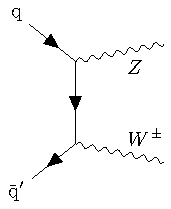
\includegraphics[page=1,width=0.22\textwidth]{figures/FeynmanDiagrams/WZNLOfeynman.pdf}
   \includegraphics[page=2,width=0.22\textwidth]{figures/FeynmanDiagrams/WZNLOfeynman.pdf}
   \includegraphics[page=3,width=0.22\textwidth]{figures/FeynmanDiagrams/WZNLOfeynman.pdf}
  \caption[Contributions to the $\pp\to\WZ$ process at NLO]{
    Contributions to the $\pp\to\WZ$ process at NLO. The leftmost diagram is the Born
    contribution, which is part of the LO calculation. The real-emission diagram
    is shown in the center, and the loop contribution is far right. The cross section
    is proportional to the square of the sum of amplitudes shown, which at 
    $\mathcal{O}(\alpha_s)$ includes the square of the Born and real-emission diagrams
    and the interference of the loop and Born diagrams.
  }
 \label{fig:WZNLO}
\end{figure}

Diboson processes inclusive in the number of jets have recently become available 
at next-to-next-to-leading order (NNLO)~\cite{Grazzini:2017mhc}. These calculations
have an additional layer of complication due to the more complex cancelling of
divergences between double loop, double real-emission, and combined real-emission
and loop contributions. They are not yet automated,
partially because not all two-loop amplitudes in the SM are known.
Combining these predictions with hadronization functions,
discussed in the following sections, is also not yet accomplished for diboson
processes. In this thesis, we use NNLO cross section calculations to 
correct the predicted yields of NLO simulations for diboson processes.

\section{Monte Carlo integration and event unweighting}

As referenced in the previous section, calculations of physical
quantities involve integrations of the amplitude over the relevant phase space
for the scattering process. 
The phase space integration in Equation~\ref{eq:meint}
is an integration over the quantum numbers and four-momenta of all particles 
considered. The integration is often complex and rarely solvable analytically.
The MC integration algorithm
was first formally developed in the late 1940s as part of the Manhattan project,
with the name derived from the eponymous casino for due to its leveraging
of random processes~\cite{10.2307/2280232}.
It is well suited for the phase space integration, because the
the uncertainty in the result scales independently of the dimensionality 
of the integration~\cite{doi:10.1002/wics.1314}. 

The MC procedure estimates 
the integral of a function $f(x_{i},\cdots,x_n\equiv\vec{x})$, defined over a volume $V^{n}$,
by tossing random random points inside a known volume
over which the function is defined, of dimension $V^{n+1}$. The volume $V^{n+1}$
from which the random numbers are drawn must fully contain 
$f(\vec{x})$, however, no further knowledge of $f(\vec{x})$ over $V^{n+1}$ is required. The function
is evaluated for the coordinates $x_i\cdots x_n$ of the random point.
If the random point is inside the volume of $f(\vec{x})$, it is accepted,
if it falls in a region of $V^{n+1}$ outside of $f(\vec{x})$ it is rejected.
As the number of points sampled $N$ grows, the ratio of the number of accepted
points to $N$ times the volume of $V^{n+1}$ approaches the integral of $f(\vec{x})$.
This is illustrated for one dimension in Fig.~\ref{fig:mcintegration}.
The error of the integration decreases proportional to $\sqrt{N}$, which
is very poor for low dimension integration ($\lesssim$4) but much better than
traditional techniques for high-dimensional problems.

\begin{figure}[htbp]
  \centering
   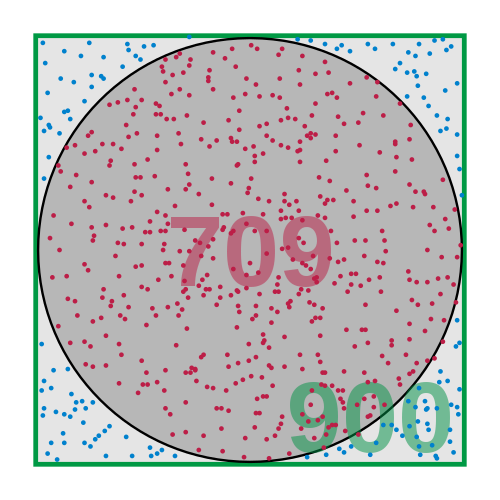
\includegraphics[width=0.6\textwidth]{figures/Simulation/MCintegration.png}
  \caption[Illustration of the principle of Monte Carlo integration]{
    Illustration of the principle of Monte Carlo integration. If the area
    of the rectangular phase space is known, the area of the circle can
    be estimated from the ratio of randomly sampled points falling
    inside or outside the volume. In this example, the ratio of accepted
    points (709, red) to the total points sampled (900) approximates the
    analytic result for the ratio of the areas, $\pi/4$.
    Reproduced under public license from Ref.~\cite{wiki:mc}.
        }
 \label{fig:mcintegration}
\end{figure}

In addition to predictions for aggregated quantities such as total cross sections
and differential rates, event-wise simulations are critical to modeling expected 
results in the realistic environment of particle physics measurements.
The MC integration approach is well-suited for this, as the procedure of randomly
sampling the integrand over a phase space can be leveraged to draw events from
the distribution. In this procedure, specific realizations of particle states,
including quantum numbers and four momenta, are sampled from
the possible outcomes with rate proportional to the probability for production,
given by the phase space and squared amplitude of Equation~\ref{eq:meint}.

\section{Event simulation for experimental analysis}
Calculations using the previously described techniques, which 
truncate at a specific order of perturbation theory and treat quarks and gluon 
as free particles, are referred to as ``fixed-order'' calculations.
For the $\pp\to\WZ\to\ell\nu\ell'\ell'\jet\jet$ process, 
Equation~\ref{eq:meint} can be used to compute observables at fixed order for the underlying
subprocesses, e.g., when a $\Pq\Pq'$ interaction takes place and
$\jet\jet=\Pq\Pq''$. 
This parton-level process can be used to derive useful predictions,
however, events containing free partons and leptons 
do not offer a full picture of the objects that interact with the CMS
detector. High-energy partons radiate quarks and gluons or split to $\Pq\Paq$
pairs, reducing their energy until they reach the energy scale of hadronization \lqcd.
Similarly, leptons can radiate photons, which can subsequently pair produce photons.
Both effects are considered in the QCD and QED showers, which simulate successive soft
emissions of massless or nearly-massless particles.
At the scale {\lqcd}, the free partons form hadrons. Long lived hadrons interact with the detector,
whereas shorter-lived hadrons decay to neutrinos, leptons, or other hadrons before interacting.
These considerations, combined with additional \pp interactions in a single LHC bunch crossing,
as well as multiple parton-parton interactions in a single \pp collision, contribute to the full $\mathcal{O}(1000)$
particle multiplicity measured in the CMS detector per event. The properties and kinematic
distributions, as well as their interactions with the CMS detector, must be well-understood
for a full simulation of a realistic event.

\subsection{The parton shower and matching to matrix element calculations}
The shower allows radiations at low transverse momentum
and angular separation to be summed to all orders in perturbation theory. It is based on the
observation that the matrix elements $\mathcal{M}_{a\to b}$ and $\mathcal{M}_{a\to bc}$ are related
as $\mathcal{M}_{a\to bc} \approx f(P_{b \to bc})\mathcal{M}_{a\to b}$
in the limit where $\pt^{b}$ and the angular separation $\theta_{bc}$ is small~\cite{Peskin:1995ev}.
In this expression, $f(P_{b \to bc})$ is an exponentially decreasing function, strictly less than one, 
of the splitting function $P_{b \to bc}$ for the particle $b$ to $bc$.
Thus, in this soft and collinear limit, additional radiation can be interpreted as a 
matrix element for production of the state $b$, and a factorizable probability for the 
incoming partons and final state particles---quarks, gluons,
leptons, and photons---to radiate or pair convert. 
The MC techniques described previously are well suited
for event-wise simulation of the shower, because random numbers can 
be linked to probabilistic parton splitting.

The shower is most important for QCD
radiation, because gluon radiations and splittings occur with high probability. Therefore,
it is generally referred to as a ``parton shower,'' even though photon radiation is also considered.
The QCD splitting functions $P_{b\to bc}$ 
are equivalent to the Altarelli--Parisi functions used in the determination of the PDF,
thus, they are well established. 
The process is followed iteratively,
allowing subsequent radiations to evolve the state $a$ into a state $a+X$, where
$X$ represents additional quarks or gluons. In this way, the parton shower
evolves inclusive matrix element calculations, which give predictions
for \textit{at least} $n$ partons ($n=2$ for \WZjj production), 
to be evolved to exclusive predictions for \textit{exaclty} $n$ partons
or clustered jets.

If the matrix element calculation includes outgoing partons, care must
be taken ovoid overlap between the matrix element and shower components of the event.
At LO, this is trivially accomplished by limiting the $\pt$ of partons 
generated by shower splittings to be less than those generated by the matrix 
element---otherwise the harder shower emission would duplicate a possible
configuration with harder matrix element partons and soft shower radiation,
and the contribution would be double counted. 
This procedure, referred to as shower matching, is more complex for NLO
calculations, because shower radiation from the Born diagrams
(Fig.~\ref{fig:WZNLO}, left) overlaps the contribution of radiation from
the real-emission diagram (Fig.~\ref{fig:WZNLO}, center). Two techniques
were developed to resolve this conflict and enable showered and hadronized NLO 
predictions: the POWHEG~\cite{Nason:2004rx,Frixione:2007vw} and the 
MC@NLO~\cite{Frixione:2002ik} approaches.

The MC@NLO approach uses an analytic calculation of the parton shower to correct
the matrix element predictions per event. This expected contribution is subtracted
from the matrix element events, modifying the kinematics. The stochastic parton
shower is then applied to the corrected events, which are not physically meaningful
without the shower. The combined matrix element plus shower events, however, are accurate to NLO in QCD.
The POWHEG technique takes a converse approach. It corrects the 
matrix element events to account for the parton shower-like behavior at low
energy. The parton shower is applied to the corrected events, but any shower radiation harder
than the real-emission matrix element is vetoed in favor of the matrix element contribution.
We study both techniques for the $\pp\to\WZ$
process, and find agreement for inclusive variables.

In addition to more accurate cross section predictions,
an NLO calculation has the advantage of describing additional parton
contributions to the state with matrix-element-level calculations, via
the real emission diagrams. Because calculating the virtual contribution contributing at NLO
is a major challenge, it is natural to consider a way to combine the Born
and real-emission contributions without relying on difficult loop diagram calculations.
However, it is important to reiterate that matrix element calculations at a fixed
order in perturbation theory are inclusive quantities. 
Tree-level diagrams that contribute at a higher order of $\alpha_s$ cannot be naively
calculated and added to the prediction, without including the virtual contribution,
that effectively regulates the relative contributions of the two. 
The parton shower prescription allows the inclusive prediction to be evolved into 
an exclusive one, with a prescription to determine if a state remained a $n$-parton
state or evolved to an $n+1$-parton state. Techniques known as matrix element merging
exploit the parton shower paradigm to combine tree-level contributions with 
additional partons. In this approach, the parton shower determines how the
inclusive state evolves from an inclusive to exclusive state of many partons,
and the tree-level matrix elements are used to correct the distributions of the
multi-parton states.
This idea has also been extended to NLO calculations, avoiding the 
double virtual and real-virtual contributions in the \FxFx~\cite{Frederix:2012ps}
and MINLO~\cite{Hamilton:2012np} algorithms.

We use LO merging, via the MLM merging algorithm~\cite{MLMmerging} 
implemented in \MG, to simulate the \QCDWZ process. By merging
contributions to \WZ production with up to three outgoing partons, we achieve
an accurate description of the two-jet kinematics of the \WZjj state without
relying on computationally prohibitive higher-order calculations. 
We also exploit NLO-merging, 
but the number of outgoing partons that can be simulated is lower. 
The \FxFx algorithm is used for alternative simulations of the \QCDWZ
process, for background diboson process, and for some backgrounds with 
top quark production.

\subsection{The underlying event, hadronization, and decay}
Hadronization refers to the transition from colored partonic states to the 
colorless hadronic states that populate the low-energy physical world. 
In general, the distributions of the total momentum of hadrons forming jets is approximately
described by the momentum distribution from perturbative calculations of partons,
so fixed-order calculations are still useful for predictions about the \WZjj state.
Generic parton-to-hadron fragmentation functions
are also sometimes used to estimate the transition from partons to hadronic jets
to improve on these calculations.
However, a much richer picture of hadron formation 
is obtained by simulating hadronization from the
multi-parton state of the remnants of the interacting protons
and the parton shower evolved to to a cutoff scale
$\sim$\lqcd~\cite{Buckley:2011ms}. 

Partons do not hadronize
individually, rather, they interplay to build colorless systems.
To good approximation, the hadronization process can be considered universal, that is,
the formation of hadrons is independent of the production mechanism of the
partonic state, only on its configuration at the hadronization scale.
Two models are used in general-purpose MC generators: the cluster model,
implemented in {\Sherpa} and \Herwig, and the Lund string model, implemented in
\Pythia. The cluster model is based on forming clusters of colorless quarks
at the shower cutoff scale, after splitting gluons to {\Pq\Paq}. As demonstrated
by Amati and Veneziano in 1979~\cite{Amati:133141}, color singlets at the cutoff scale have
a mass distribution independent of the energy scale of the production process.
The color singlet clusters are then decayed into hadrons according to the available phase space.
The string model seeks to model the process of confinement more directly. 
The $\Pq\Paq$ pairs are consider connected by confinement strings
with potential energy proportional to the separation in the quark rest frame, $V=\kappa z$.
Observationally, $\kappa\approx 1\GeV/\mathrm{fm}$, which is consistent with calculations in 
lattice QCD. As the $\Pq\Paq$ pairs are separated, the energy increases, and it may
be energetically favorable to snap the string with new $\Pq'\Paq'$ pairs from the vacuum,
as illustrated in Fig.~\ref{fig:hadronization}.
High energy gluons show up as kinks in the string, which give rise to more
hadron formation in the gluon direction. The process continues
until the color singlet pairs, or colorless $\Pq\Pq\Pq$ groups, are not
energetic enough to break the confining string and form hadrons.

\begin{figure}[htbp]
  \centering
   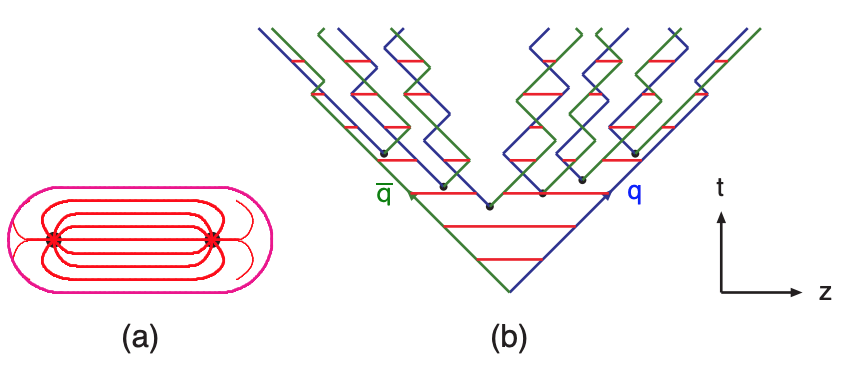
\includegraphics[width=0.6\textwidth]{figures/Simulation/StringHadronization.png}
  \caption[Illustration of hadronization in the string model]{
    Illustration of hadronization in the string model. Field
    lines from gluon exchange lead to a string-like linear force
    between $\Pq\Paq$ pairs (a). As the energy of the string increases,
    it is energetically favorable to produce new $\Pq'\Paq'$ pairs (b).
        }
 \label{fig:hadronization}
\end{figure}

The cluster and string models both require input parameters derived from 
data, especially from measurements of jet formation in \EE collisions at LEP.
The string model of \PYTHIA is often seen to perform slightly better, however,
it is dependent on a greater number of parameters derived from data.
Good agreement is seen between these models for the \WZjj state considered in this analysis.
The simulation of the parton shower
and matrix element merging, discussed in the previous section, 
have more impact on the dijet kinematics of \WZjj events, which are critical
to the analyses considered in this thesis, 
than does hadronziation process.

Multi-parton interactions (MPI) and pileup are also important for a
realistic picture of particle formation in LHC collisions. The MPI is primarily
soft; it does not generally result in easily identifiable jets, but
it impacts the total energy transfer in a scatter event and affects the color
connections of the scatter partons and proton remnants, leading to a more complex
hadronization stage~\cite{Buckley:2011ms}. The MPI is modeled in \Pythia, with parameters tuned 
by the CMS experiment using 7 and 8\TeV data as presented in Ref.~\cite{Khachatryan:2015pea},
referred to as the CUEP8M1 tune. Pileup is simulated using large datasets of 
events of elastic and low-energy transfer \pp scattering events, referred
to as minimum bias events, simulated with \PYTHIA 8. Events are sampled randomly
from the dataset and mixed into the simulated sample of hard-scattering events
such that the number of pileup events matches that observed in data.

Hadron decays are simulated with a combination of theoretical models,
including simple matrix element calculations for the light mesons and tau,
and observational data from experimental measurements as tabulated
by the Particle Data Group in Ref.~\cite{Tanabashi:2018oca}. Spin-dependent
decays depend on the production mechanism of the particle. 
The production and decay spin correlations are taken into account by using \textsc{MadSpin}~\cite{Artoisenet:2012st} 
together with \PYTHIA for simulations used in this analysis.

\subsection{Detector simulation}

To build a dataset of realistic collision events, used to guide this
analysis and model expected signal and background distributions,
the interactions of the particles that reach
the CMS detector in the active and inactive volume are simulated using a
detailed model in the \GEANTfour program~\cite{GEANT,Geant2}.
\GEANTfour includes a large set of physics models over an energy range
from several eV to TeV, and it effectively serves as a repository of the known
set of interactions of particles with matter.
The paths of primary and secondary particles through the CMS detector
are traced by \GEANTfour, using the MC method to determine interactions
according to their probabilities. Decays of semi-stable particles 
are calculated and their decay products are tracked. Energy deposits
and hits in the detector are recorded and transmitted to customized digitization software.
The digitized information, designed to accurately emulate the real CMS 
electronics, is fed through the same reconstruction algorithms as real data. 

The performance
of the detector modeling and digitization have been tuned and validated using
both test beam~\cite{CMS-DP-2018-045} and collision data~\cite{Banerjee:1345317}.
Nonetheless, differences in the simulated and collected data are unavoidable. They 
arise due to, e.g., inactive regions in the detector, shifts in the detector alignment,
and radiation damage. Differences in data and simulation efficiencies are corrected
using known quantities, such as the lepton kinematics from $\cPZ$ decays or jet
energies in dijet events. These corrections are generally at the percent level. As discussed
in Chapters~\ref{ch:analysis} and \ref{ch:results}, the agreement between data
and MC simulation is excellent for most processes considered in this result.

\section{Simulations of \WZjj production}

The primary generators used in this analysis are \MG and \POWHEG 2.0 for simulation
of the hard-scattering interaction at LO or NLO, and \PYTHIA 8 for parton
showering and hadronization. The specific samples used for background processes
are discussed in Chapter~\ref{ch:analysis}. Because the MC simulations are fudamental
to distinguishing the EW- and QCD-induced contributions to \WZjj, particular
care is taken in studying the simulation of these processes.

Standard techniques to evaluate the uncertainties of MC simulations involve
varying the parameters of the PDF fit and the scale of the {\muF} and {\muR} parameters,
as discussed in Chapter~\ref{ch:analysis}. 
%Because {\muF} and {\muR} arise due to the truncation
%Of the perturbation series and the division between hard and soft scales,
%They can also be used as a probe of the impact of these choices on the calculation.
It is well established that these approaches offer a probe of the precision
of a perturbative calculation. However, the extent to which they represent
an uncertainty that can be interpreted in a statistical sense, and that fully
covers the impacts of additional missing orders of the calculation, are unknown.
In addition, additional parameters in a full simulation, such as the tuning
of the shower and hadronization to data, are not captured by this approach.
Even for fixed-order calculations, several parameters must be input to the calcultion,
including the functional form of the {\muF} and \muR, the couplings, and particle masses and
widths. 

A useful approach to obtain a broad picture of the uncertainty of theoretical
predictions for a process is to compare results between different calculations.
In principle, all differences should be traceable to specific choices in the calculations.
However, probing all possible sources of differences in a hadronized prediction is a very
tedious process. It is essential when understanding sources of disagreement, but
may not be necessary when demonstrating that broadly different models of, e.g., parton
shower and hadronization, give similar results.
For the work presented in this thesis, we use comparisons of MC generators to demonstrate that the 
features of the \EWWZ and \QCDWZ processes that we exploit for this analysis 
are theoretically well understood.
Much of this work was performed
in collaboration with experts in the theoretical community at the Les Houches 2017
workshop, and reported in Ref.~\cite{leshouches2017}.

Following this work, results are presented for the following event selection,
referred to as the fiducial region.

\begin{itemize}
\item All charged leptons are required to have
    \begin{align}
        \label{eq:cut1}
         \pt^{\ell} >  20\GeV,\qquad |y_{\ell}| < 2.5.
    \end{align}
\item For the leptons of opposite charge and same flavour, an invariant mass cut to single out the $\PZ$ boson resonance is applied:
    \begin{align}
        \label{eq:cut2}
         76\GeV < m_{\ell^{+}\ell^{-}} < 106\GeV.
    \end{align}

\item hadronic or partonic particles are cluster into jets using the anti-$\kt$ algorithm~\cite{Cacciari:2008gp} with radius parameter $R=0.4$.
      At least two jets are required to have
        \begin{align}
        \label{eq:cut3}
         \pt^{\jet} >  30\GeV, \qquad |y_{\rm j}| < 4.7, \qquad \Delta R_{\jet \ell} > 0.4,
        \end{align}
        %
        and are called tagging jets.
\item On the two leading tagging jets, typical VBS cuts are applied:
        \begin{align}
        \label{eq:cut4}
        \mjj >  500\GeV,\qquad \abs{\detajj} > 2.5.
        \end{align}
\end{itemize}
\subsection{Predictions from fixed-order calculations}

Calculations of the \EWWZ process at NLO in QCD were first performed
some over ten years ago~\cite{Bozzi:2007ur}, however, only recently have these
results been implemented in a form that is compatible with parton shower and 
hadronization generators~\cite{Jager:2018cyo}. Recent preliminary
results considering both NLO EW and QCD effects for \WZjj production are also limited to fixed order.
Therefore, it is necessary to consider fixed-order results in order to study 
the best available predictions for this process. Moreover, the additional
complications of showered and hadronized events can complicate efforts to
establish the relative agreement of generators. 

\begin{figure}[htbp]
  \centering
   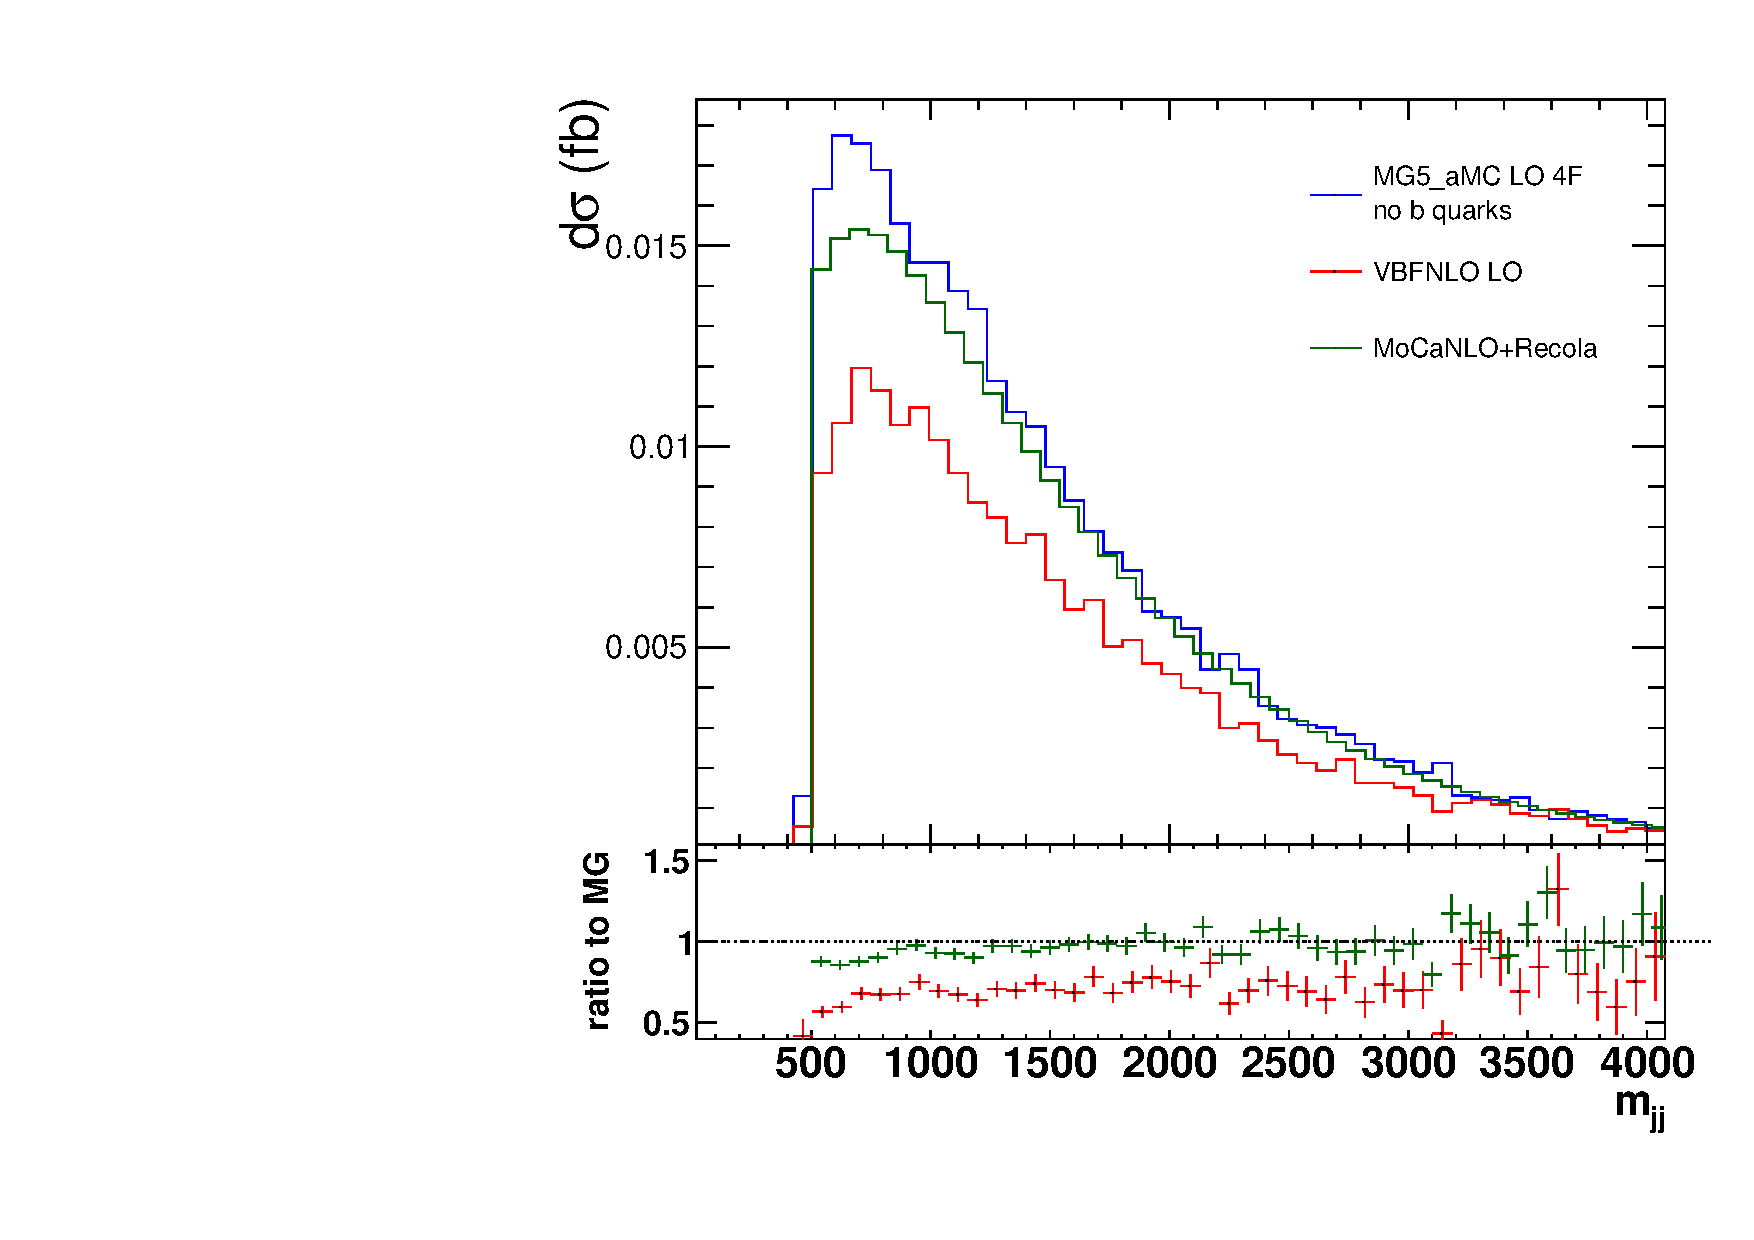
\includegraphics[width=0.49\textwidth]{figures/Simulation/mjj_FO_untuned.pdf}
   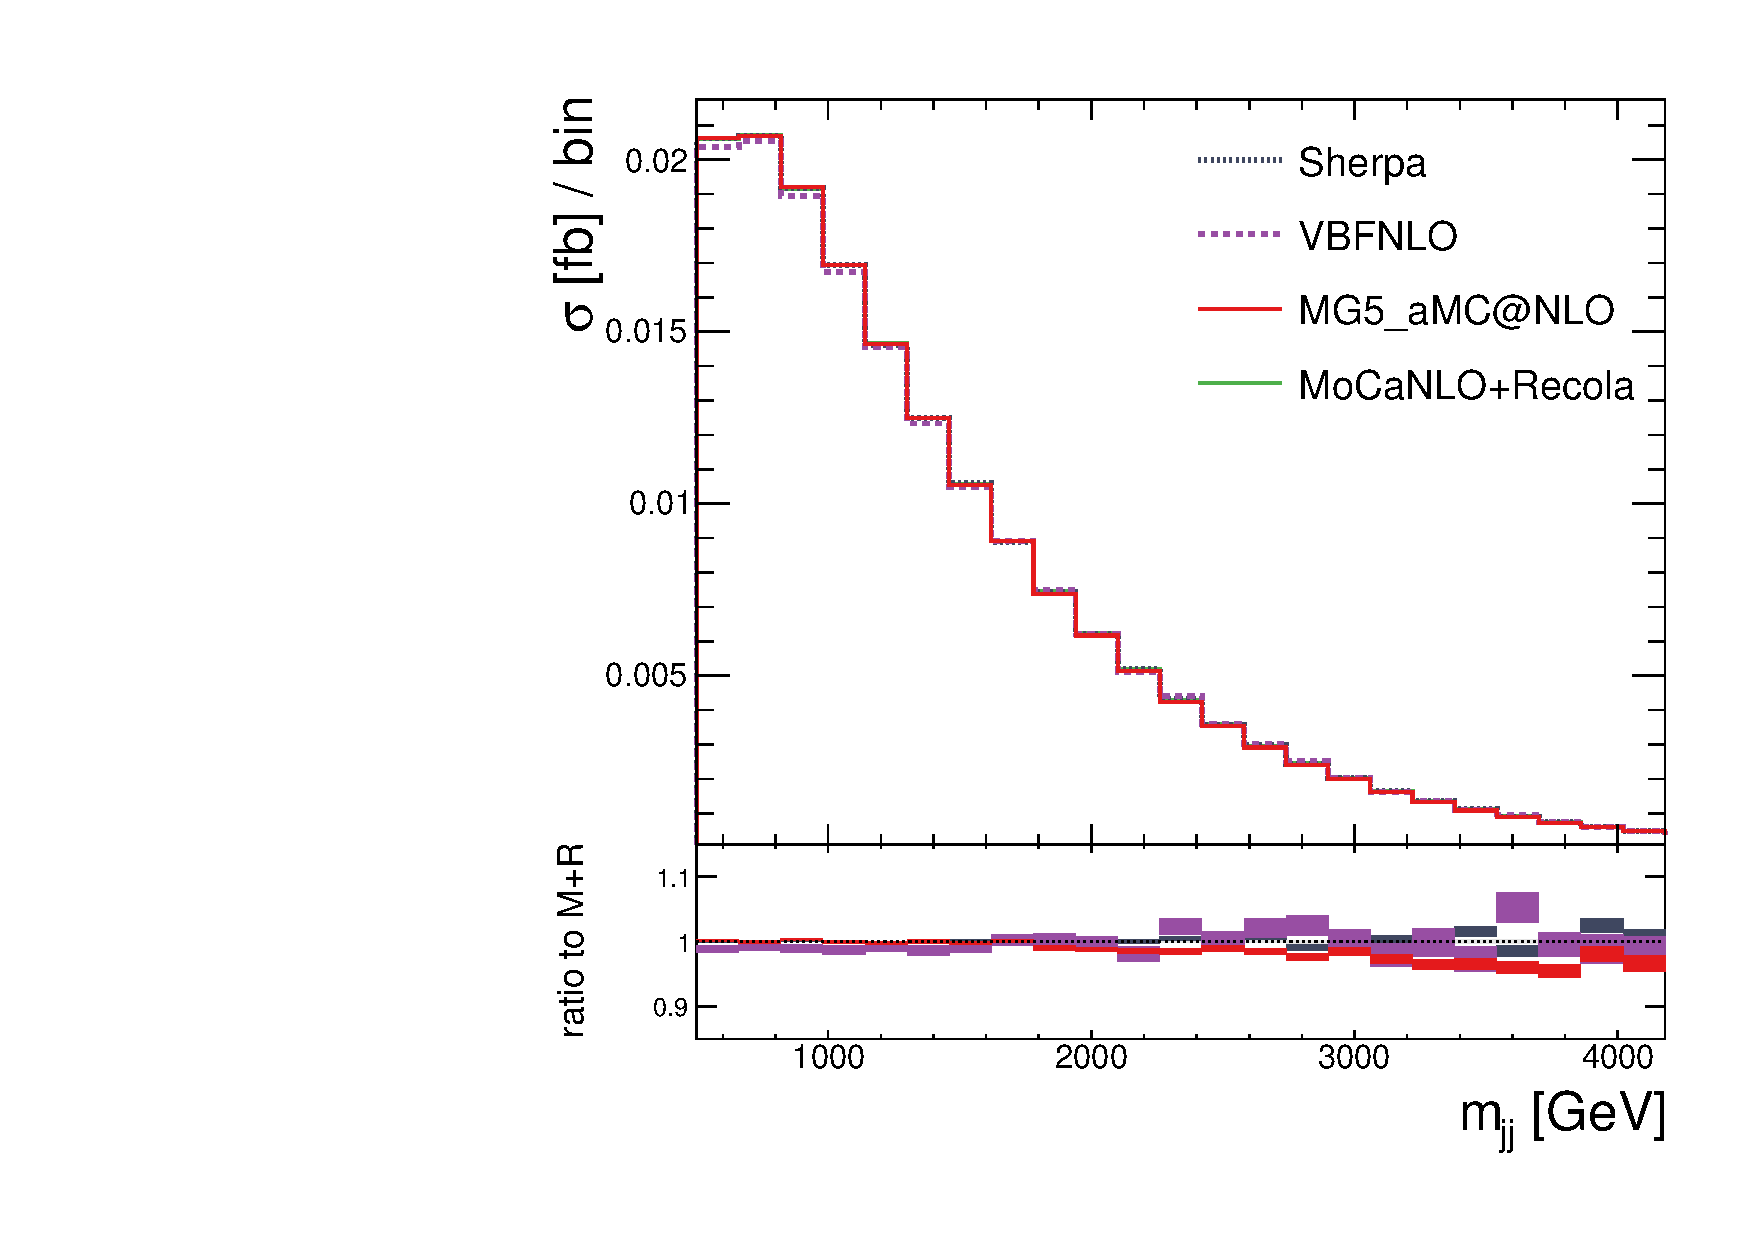
\includegraphics[width=0.49\textwidth]{figures/Simulation/mjj_FO_tuned.pdf}
  \caption[The fixed-order prediction for $\mjj$ from \MG, {\Sherpa}, {\VBFNLO}, and {\Moca} at LO]
  {
    The fixed-order prediction for $\mjj$ from \MG, {\Sherpa}, {\VBFNLO}, and {\Moca} at LO
    for the \EWWZ process. The left comparison is made using the default settings
    of all input parameters for the public MC programs. The right plot is shown
    with parameters tuned to the values given in Ref.~\cite{leshouches2017}.
        }
 \label{fig:FOWZcomparisons}
\end{figure}

For this reason, we first consider comparisons of the \EWWZ process at fixed order. 
Because the process has no $\alpha_s$ couplings at LO, the 
calculation has almost no $\muR$ dependence.
The $\muF$ dependence is also relatively low, $\mathcal{O}(10\%)$
leading order. Furthermore, the NLO corrections to the cross section are small,
the $k$-factor $k\equiv \sigma_{NLO}/\sigma_{LO} = 0.98$ in the fiducial region
defined in Equations~\ref{eq:cut1}-\ref{eq:cut4}, calculated with 
VBFNLO~\cite{VBFNLO}. Nonetheless, the process has a significant dependence on
the masses, widths, and couplings of the particles used in the calculation,
as demonstrated in Fig.~\ref{fig:FOWZcomparisons}. The Les Houches study demonstrated
that discrepancies may arise at fixed-order when these parameters are not controlled,
however, when using a common,  
well-motivated parameters (following the best-available measurements), 
excellent agreement is obtained. 
Because most settings can be determined in an objective way, we do not consider
such differences to constitute additional uncertainty in modeling this process.

\subsection{Hadronized predictions and fully-simulated events}

We also study the modeling of the \EWWZ process using hadronized events. 
The results are largely consistent with the studies at fixed order;
agreement is seen across a broad range of generators for leptonic variables,
or kinematic variables of the two-jet system. 
Specifically, the variables $\mjj$, $\etajj$, and
$\etas\equiv\zepl$ (sometimes referred to as the "Zeppenfeld variable") are
all well described, and can be exploited in this analysis with limited uncertainty.
Variables depending on more than
three clustered jets, produced purely by the shower and hadronization for the MCs we consider, 
can have significant differences. This is expected: the parton shower and hadronization
of {\Sherpa}, \Herwig, \MG, and \Pythia use different models and different tuned parameters.
Because many are phenomenological, it is difficult to constrain them extensively.
We acknowledge a higher modeling uncertainty for such variables, and seek to avoid
relying on their simulation in this analysis. Example distributions with large
and small shower dependence are shown in Fig.~\ref{fig:ewwzHadronization}.

\begin{figure}[htbp]
  \centering
   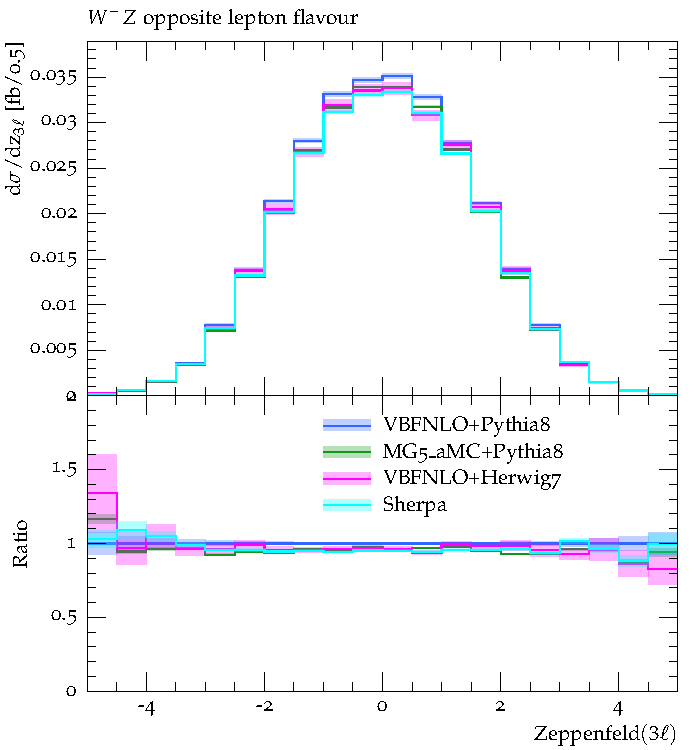
\includegraphics[width=0.49\textwidth]{figures/Simulation/LH_VBFNLO_WmZ_OF_zep3l.pdf}
   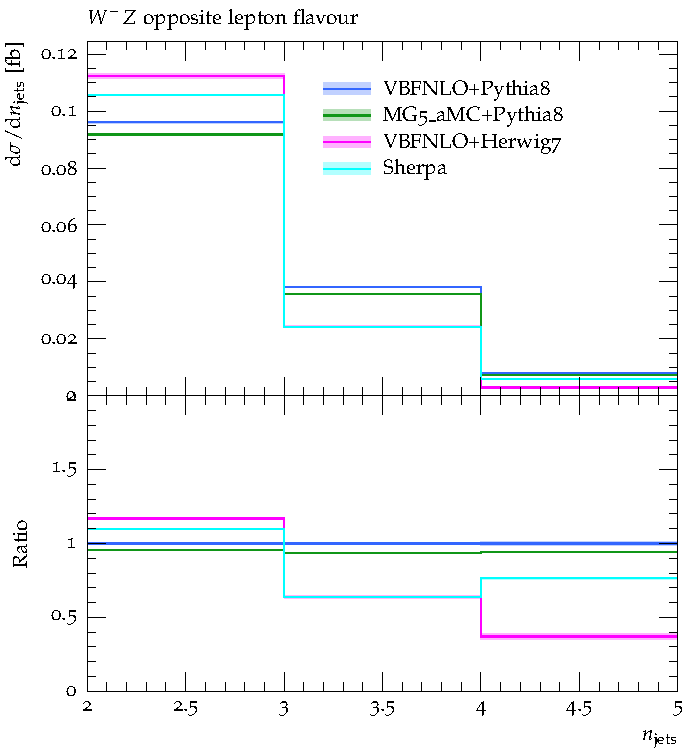
\includegraphics[width=0.49\textwidth]{figures/Simulation/LH_VBFNLO_WmZ_OF_nJets.pdf}
  \caption[Comparison of predictions for \EWWZ production including hadronization effects]
  {
    Predictions for EW $\PW^{-}\cPZ\to\EE\mu^{-}\PAGnGm$, production, including the parton
    shower and hadronization. Variables well described by the fixed-order calculation,
    including $\etas$ (left), are not significantly impacted by the shower and hadronization.
    Variables with a large dependence on shower and hadronization, including the number
    of jets with $\pt > 30\GeV$ (right), show larger variance between MC generators.
        }
 \label{fig:ewwzHadronization}
\end{figure}

The MC simulation used to guide this analysis and to extract results is generated
with \MG~v2.4.2. We use the default dynamic scale choice and input parameters of \MG.
This choice was made for practical reasons, though we validate that only the total
cross section, but not sensitive distributions, is affected by this choice, as
illustrated in Fig.~\ref{fig:ewwzMGLH}. The cross section with this configuration
is about 10\% lower than with the Les Houches settings. The \EWWZ cross section 
measurement relies on shape predictions, but not on the predicted cross section,
so this difference is not considered as an uncertainty.
The shapes of two-jet variables
are only majorly impacted by the corrections, is shown in Fig.~\ref{fig:ewwzPOWHEG}
for \EWWZ production at NLO with parton shower and hadronization from \POWHEG~\cite{Jager:2018cyo}
These comparisons give us confidence that differential predictions for \EWWZ production
are well understood.
The $k$-factor in this region is slightly lower than the VBFNLO fixed-order prediction.

\begin{figure}[htbp]
  \centering
   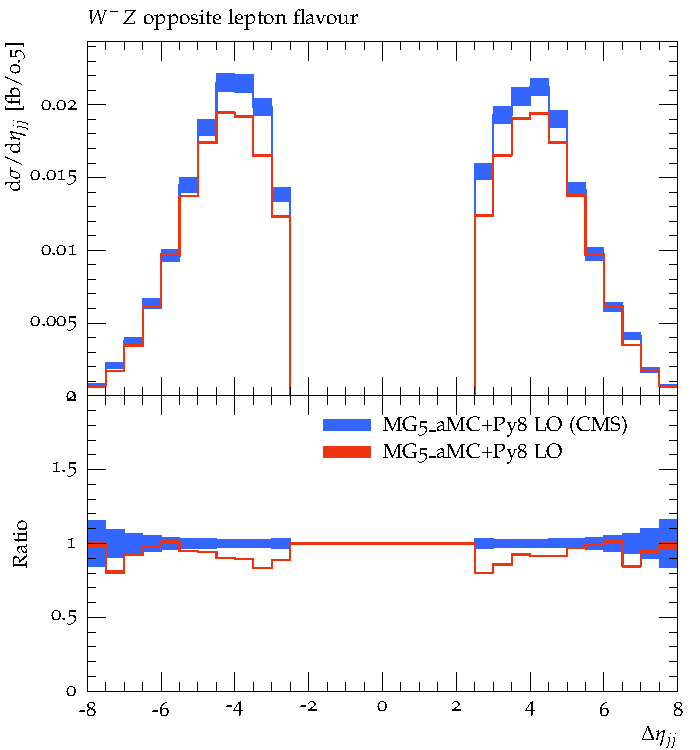
\includegraphics[width=0.49\textwidth]{figures/Simulation/MGLH_WmZ_OF_dEtajj.pdf}
   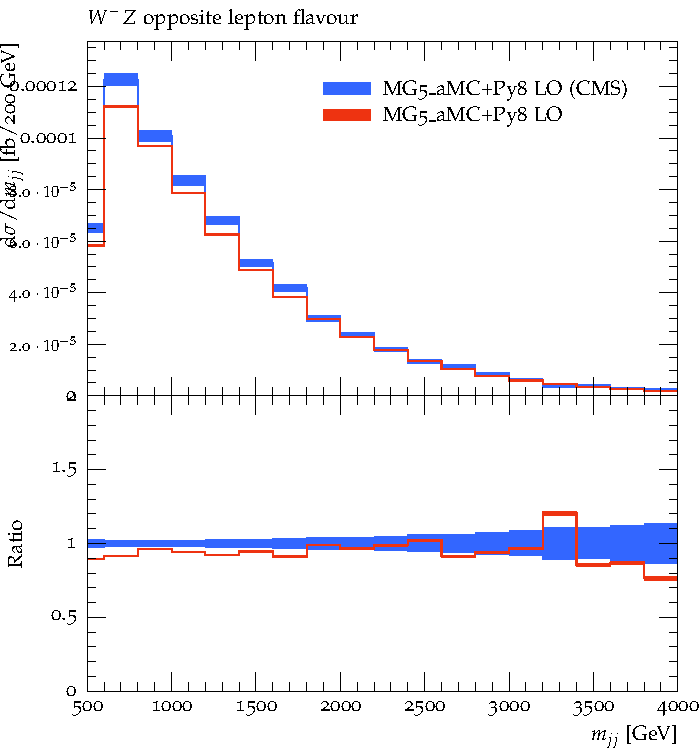
\includegraphics[width=0.49\textwidth]{figures/Simulation/MGLH_WmZ_OF_mjj.pdf}
  \caption[Comparison of predictions for \EWWZ using different generator configurations]
  {
    Predictions for EW $\PW^{-}\cPZ\to\EE\mu^{-}\nu_{\mu}$ production at LO in QCD simulated with
    \MG~v2.4.2 for the fiducial selection described in the text. The simulation used
    to extract results for this analysis is shown in blue. The simulation configured
    with the suggestions of the Les Houches study is shown in red.
  }
 \label{fig:ewwzMGLH}

\end{figure}
\begin{figure}[htbp]
  \centering
   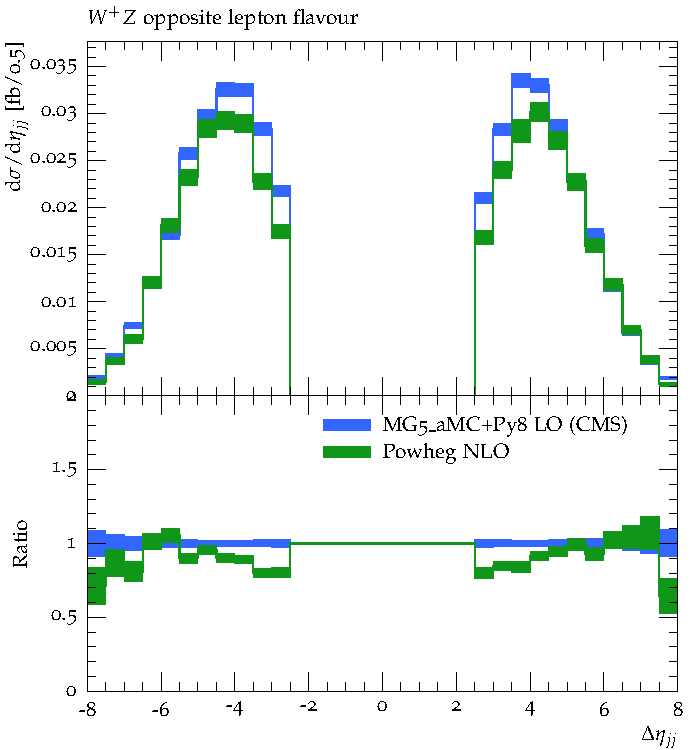
\includegraphics[width=0.49\textwidth]{figures/Simulation/POWHEGvMG_LH_WpZ_OF_dEtajj.pdf}
   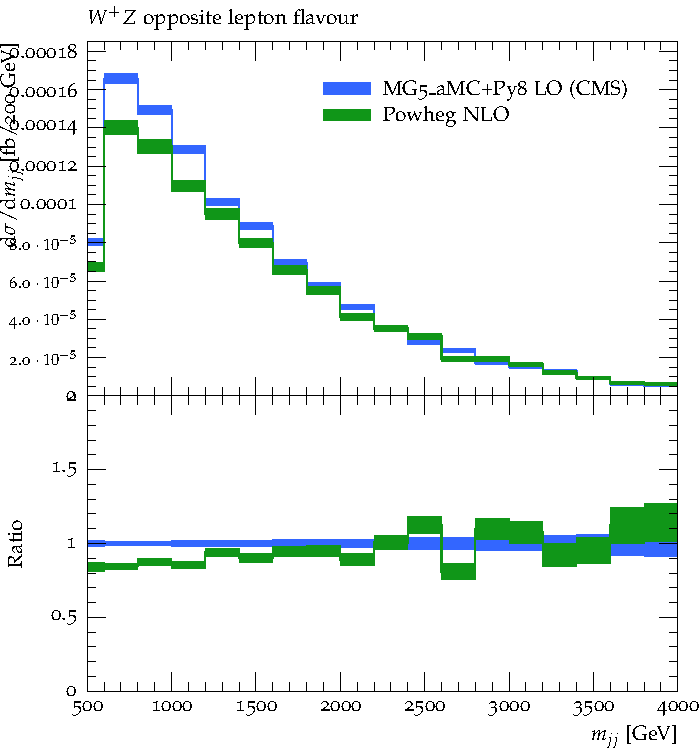
\includegraphics[width=0.49\textwidth]{figures/Simulation/POWHEGvMG_LH_WpZ_OF_mjj.pdf}
  \caption[Comparison of predictions for \EWWZ production at LO and NLO including hadronization effects]
  {
    Predictions for EW $\PW^{-}\cPZ\to\EE\mu^{-}\nu_{\mu}$ production simulated at LO with 
    \MG~v2.4.2 and at NLO with \POWHEG for the fiducial selection described in the text. 
  }
 \label{fig:ewwzPOWHEG}
\end{figure}

Because QCD-induced \WZjj production is $\mathcal{O}(\alpha_s^{2})$ it has a large
dependence on $\muF$ and $\muR$, especially at LO. Fixed-order calculations have been
performed at NLO~\cite{Campanario:2013ysa}, but hadronized simulations are computational
challenging and are therefore not considered here.
Several MC simulations of the \QCDWZ process, including parton shower and hadronization,
are considered.
The simulations are inclusive in the number of jets associated with the 
leptonically decaying \PW and {\cPZ} bosons, and therefore include 
the \WZjj contribution studied in this analysis.
The primary MC sample is simulated at 
LO with \MG v2.4.2, with contributions to \WZ production with up to three outgoing partons 
included in the matrix element calculation. 
The different jet multiplicities are merged using the MLM scheme~\cite{MLMmerging}.
An NLO sample from \MG v2.3.3 
with zero or one outgoing partons at Born level, merged using the \FxFx scheme,
and an inclusive NLO sample from \POWHEG2.0~\cite{Melia:2011tj,Nason:2004rx,Frixione:2007vw,powheg:2010}
are also considered. 
The LO MC with MLM merging, referred to as the MLM-merged sample, 
is taken as the central prediction due its inclusion of
\WZ plus three-parton contributions at tree level, which are relevant
to \WZjj production.
The other samples,
which are used to access the modeling uncertainty in the \QCDWZ process,
are referred to as the \FxFx-merged
and the \POWHEG samples, respectively.

The scale choice and input parameters are set to the default values of the respective generators.
Due to the large scale dependence, the predicted cross sections for the $\WZjj$ state
differ by up to 20\% across the three MC generators considered. 
However, as for \EWWZ, we are most concerned with the differential
predictions for the process, because the total rate of \WZ production can be constrained
by the data. Predictions for these MC generators, normalized to the prediction of \MG
in after the two-jet selection, are shown for variables sensitive 
to the \EWWZ process in Fig.~\ref{fig:qcdwzHadronization}, where some 
differences are expected due to the parton shower schemes. Disagreement between
predictions is largely within the theoretical uncertainties considered. The 
estimation of these uncertainties, and the additional uncertainty we derive
from these comparisons after exploiting the data to constrain the 
predictions, are discussed in Chapter~\ref{ch:analysis}. 

\begin{figure}[htbp]
  \centering
   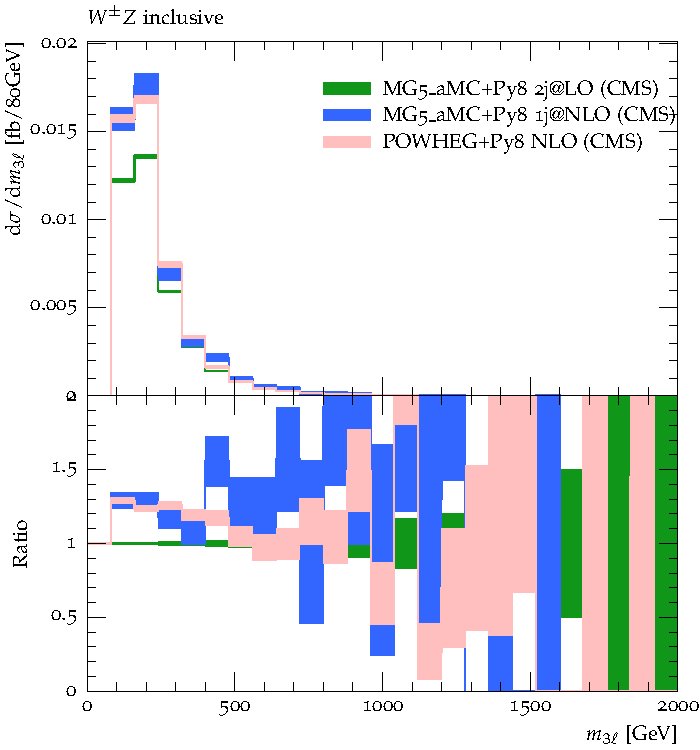
\includegraphics[width=0.49\textwidth]{figures/Simulation/QCDWZ_Mass3l.pdf}
   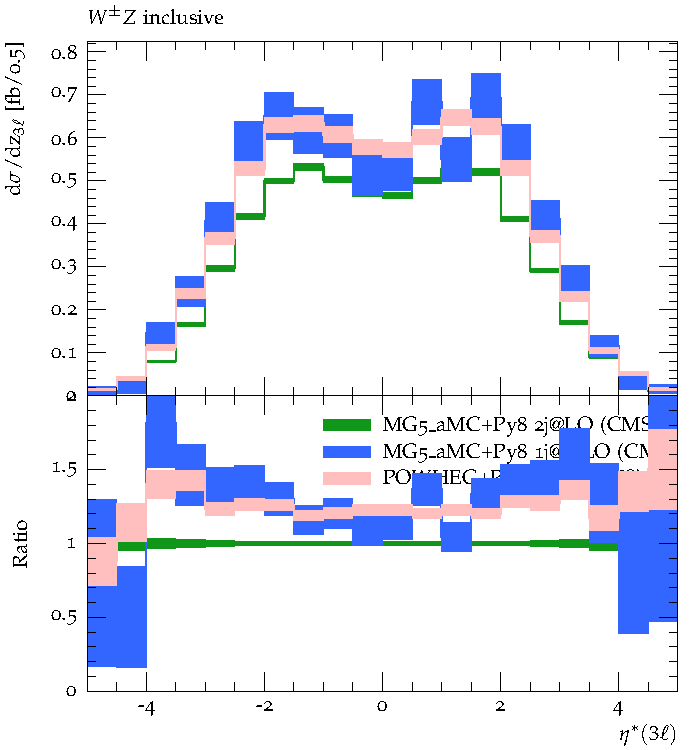
\includegraphics[width=0.49\textwidth]{figures/Simulation/QCDWZ_zep3l.pdf}
   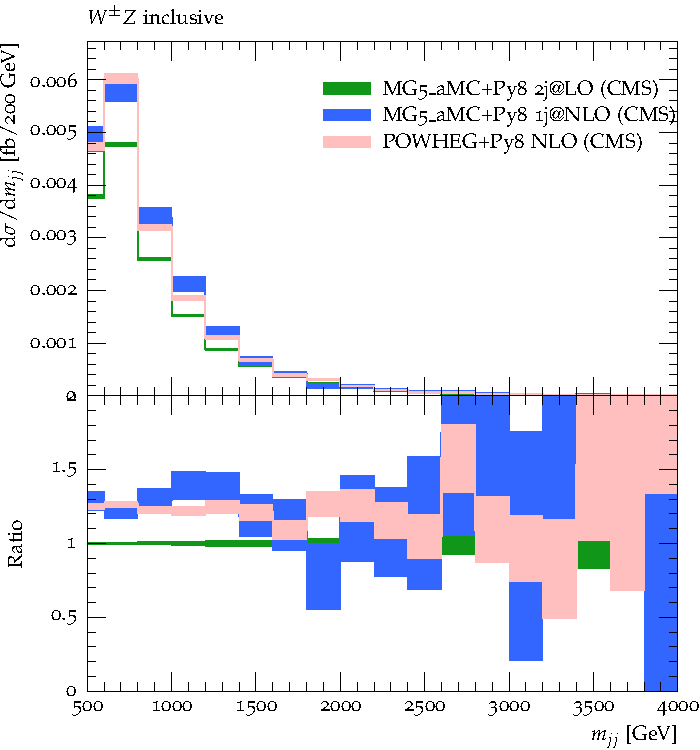
\includegraphics[width=0.49\textwidth]{figures/Simulation/QCDWZ_mjj.pdf}
   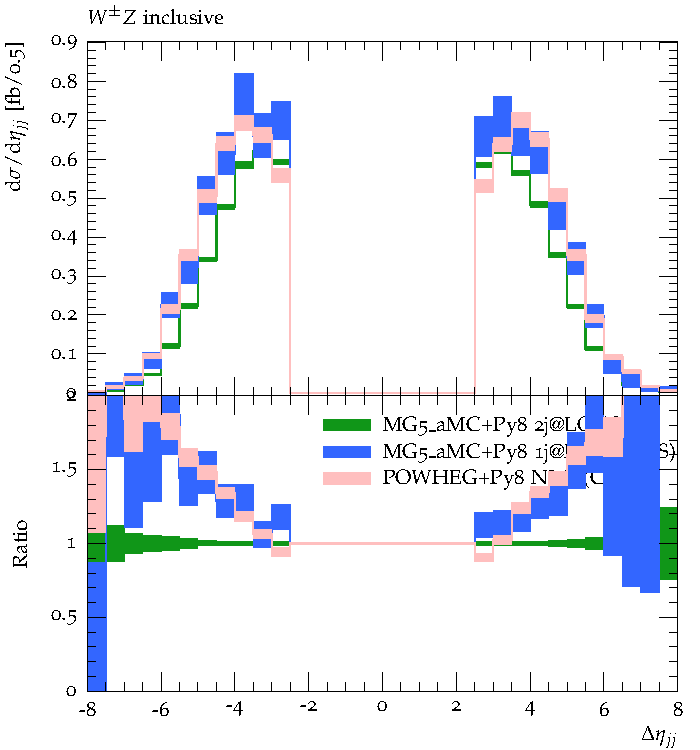
\includegraphics[width=0.49\textwidth]{figures/Simulation/QCDWZ_dEtajj.pdf}
  \caption[Comparison of predictions for \QCDWZ production including hadronization effects]
  {Comparison of predictions for the \QCDWZ process using the POWHEG, \MG MLM- and \FxFx-merged samples 
  in the fiducial region described in the text. The samples are normalized to the cross section
  from \MG after selecting \WZjj events.}
 \label{fig:qcdwzHadronization}
\end{figure}
